\documentclass[a4paper]{report}

\usepackage{amsmath,amssymb,stmaryrd,latexsym}
\usepackage{titlepic}
\usepackage{syntax}
\usepackage{alltt}
\usepackage{graphicx}   % Including Graphics
%\usepackage{verbatim} 
\usepackage{spverbatim}
\usepackage{alltt} 
\usepackage{xspace} 
\usepackage{listings} 
\usepackage{ifthen}
\usepackage{adjustbox}
\usepackage{xhfill}% http://ctan.org/pkg/xhfill
\usepackage{color}
\usepackage{fancybox}
\usepackage{fancyvrb}
\usepackage{fixltx2e}
\usepackage[multiple]{footmisc}
\usepackage{grammar-defns}  %% Generated by Obelisk

\newsavebox{\FVerbBox}
\newenvironment{FVerbatim}
 {\VerbatimEnvironment
  \begin{center}
  \begin{lrbox}{\FVerbBox}
  \begin{BVerbatim}}
 {\end{BVerbatim}
  \end{lrbox}
  \fbox{\usebox{\FVerbBox}}
  \end{center}}

\newboolean{devel}
\setboolean{devel}{false}

\lstloadlanguages{C++,VHDL}
\lstset{frameround=tttt} 
\lstset{captionpos=t}
\lstset{breaklines=true}
\lstset{escapechar=@}
%\lstset{aboveskip=2\medskipamount}
%\lstset{belowskip=1.5\medskipamount}
%\lstset{abovecaptionskip=\medskipamount}
\lstdefinelanguage{Rfsm}{keywords={type,enum,record,function,return,fsm,model,in,out,inout,vars,states,trans,itrans,on,when,with,periodic,sporadic,value_changes,event,bool,input,output,shared},morecomment=[l]{--}}
\lstdefinelanguage{ctask}{language=C,morekeywords={task,wait_ev,wait_evs,notify_ev,in,out,inout}}
\lstdefinelanguage{systemc}{language=C++,morekeywords={SC_MODULE,SC_METHOD,SC_THREAD,sc_in,sc_out,sc_inout}}

%%% Better hyphenation:
%\sloppy
\setlength{\topmargin}{0pt}
\setlength{\oddsidemargin}{0pt}
\setlength{\textheight}{600pt}
\setlength{\textwidth}{448pt}

%\Newcommand{\docdate}{\today} %%%!!!!
\newcommand{\step}{\medskip$\blacktriangleright$\xspace}

\newcommand{\version}{1.5}

\newcommand{\ie}{\emph{i.e.}\xspace}
\newcommand{\txt}[1]{\hbox{#1}}
\newcommand{\emtxt}[1]{\hbox{\em{#1}}}
\newcommand{\bftxt}[1]{\hbox{\bf{#1}}}
\ifthenelse{\boolean{devel}}{\newcommand{\note}[1]{\marginpar{\tiny #1}}}{\newcommand{\note}[1]{}}
\newcommand{\todo}[1]{\note{TODO: #1}}
\ifthenelse{\boolean{devel}}{\newcommand{\tbw}[1]{$\spadesuit$ {\bf To be written\ldots}\xspace}}{\newcommand{\tbw}[1]{}}
\ifthenelse{\boolean{devel}}{\newcommand{\tbc}[1]{$\spadesuit$ {\bf To be continued\ldots}\xspace}}{\newcommand{\tbc}[1]{}}

\newcommand{\rfsm}{RFSM\xspace}
\newcommand{\ocaml}{{\sc Objective Caml}\xspace}

\newcommand{\example}[1]{\fcolorbox{white}{lightgray}{#1}}
\newcommand{\ifname}[3]{$\mathtt{#1}_{\mathtt{#2}}\mathtt{#3}$}

%\newenvironment{example}{\medskip\noindent{\it Example :}\begin{alltt}}{\end{alltt}}

\title{RFSM User Manual - \version}

\author{J. S\'erot}

\titlepic{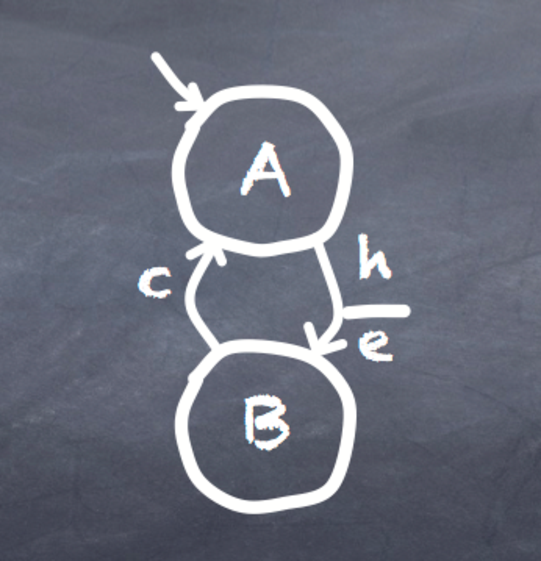
\includegraphics[width=0.5\textwidth]{figs/rfsm-logo}}
\date{}

\begin{document}

\maketitle

%\tableofcontents

\chapter{Introduction}
\label{chap:intro}

\begin{Verbatim}[commandchars=\\\{\},codes={\catcode`$=3\catcode`_=8}]
code line 1
$a_{i}$
code line 2
\textbf{boldfaced text}
a\textsubscript{i}
\end{Verbatim}

This document is a brief user manual for the RFSM toolset. It is, in its current form, very
preliminary, but should suffice for a quick grasp of the provided tools. 

\medskip
RFSM is a set of tools aimed at describing, drawing and simulating \emph{reactive finite state
  machines}. Reactive FSMs are a FSMs for which transitions can only take place at the occurence of
events.

\medskip
RFSM has been developed mainly for pedagogical purposes, in order to initiate students to
model-based design. It is currently used in courses dedicated to embedded system design both on
software and hardware platforms (microcontrolers and FPGA resp.). But RFSM can also be used to
generate code (C, SystemC or VHDL) from high-level models to be integrated to existing applications.

\medskip
RFSM is actually composed of three distinct tools :
\begin{itemize}
\item a command-line compiler (\texttt{rfsmc}),
\item a graphical user-interface (GUI) to the compiler, 
\item a library for the OCaml programming language.
\end{itemize}

These tools can be used to
\begin{itemize}
\item describe FSM-based models and testbenches,
\item generate graphical representations of these models (\verb|.dot| format) for visualisation,
\item simulate these models, producing \verb|.vcd| files to be displayed with waveform viewers such
  as \texttt{gtkwave},
\item generate C, SystemC and VHDL implementations (including testbenches for simulation)
\end{itemize}

\medskip
This document is organized as follows.
Chapter~\ref{cha:overview} is an informal presentation of the RFSM language and of its
possible usages. Chapter~\ref{cha:rfsmc} describes how to use the command-line
compiler. Chapter~\ref{cha:gui} describes the GUI-based application. Appendix A 
gives the detailed syntax of the language. Appendix B summarizes the compiler options. Appendices
C1, C2 and C3 give some examples of code generated by the C, SystemC and VHDL backends.

%%% Local Variables: 
%%% mode: latex
%%% TeX-master: "rfsm"
%%% End: 

\chapter{Overview}
\label{cha:overview}

This chapter gives informal introduction to the RFSM language and of how to use it to describe 
FSM-based systems.

\medskip
Listing~\ref{lst:rfsm-gensig} is an example of a simple RFSM program\footnote{This program is
  provided in the distribution, under directory \texttt{examples/std/single/gensig}.}. This program is
used to describe and simulate the model of a calibrated pulse generator. Given an input clock
\verb|H|, with period $T_H$, it generates a pulse of duration $n \times T_H$ whenever input
\texttt{E} is set when event $H$ occurs.

\begin{lstlisting}[language=Rfsm,frame=single,numbers=left,caption=A simple RFSM
  program,label={lst:rfsm-gensig}]
@\label{gensig-1a}@fsm model gensig <n: int> (
  in h: event,
  in e: bool,
  out s: bool)
{
@\label{gensig-1}@  states: E0, E1;
@\label{gensig-3}@  vars: k: int<1:n>;
  trans:
  | E0 -> E1 on h when e=1 with k:=1, s:=1
@\label{gensig-4}@  | E1 -> E1 on h when k<n with k:=k+1
@\label{gensig-5}@  | E1 -> E0 on h when k=n with s:=0;
  itrans:
  | -> E0 with s:=0;
@\label{gensig-1b}@}

@\label{gensig-2a}@input H : event = periodic (10,0,80)
input E : bool = value_changes (0:0, 25:1, 35:0)
@\label{gensig-2b}@output S : bool 

@\label{gensig-6}@fsm g = gensig<3>(H,E,S)
\end{lstlisting}

\medskip
The program can be divided in four parts.

\medskip The first part (lines \ref{gensig-1a}--\ref{gensig-1b}) gives a \textbf{generic model} of
the generator behavior. The model, named \verb|gensig|, has one parameter, \verb|n|, two inputs,
\verb|h| and \verb|e|, of type \verb|event| and \verb|bool| respectively, and one output \verb|s| of
type \verb|bool|. Its behavior is specified as a reactive FSM with two states, \verb|E0| and
\verb|E1|, and one internal variable \verb|k|. The transitions of this FSM are given after the
\verb|trans:| keyword in the form :
\begin{center}
  \framebox{\lstinline[language=Rfsm]{| source_state -> destination_state on ev when guard with actions}}
\end{center}
where
\begin{itemize}
\item \emph{ev} is the event trigerring the transition,
\item \emph{guard} is a set of (boolean) conditions,
\item \emph{actions} is a set of actions performed when the transition is enabled.
\end{itemize}

The semantics is that the transition is enabled
whenever the FSM is in the source state, the event \emph{ev} occurs and all the conditions in the
guard are true. The associated actions
are then performed and the FSM moves to the destination state. For example, the first transition is
enabled whenever an event occurs on input \verb|h| and, at this instant, the value of input \verb|e|
is 1. The FSM then goes from state \verb|E0| to state \verb|E1|, sets its internal variable 
\verb|k| to 1 and its output \verb|s| to 1\footnote{Boolean values \texttt{true} and \texttt{false} can
  be denoted 1 and 0 respectively in programs.}.
   
\medskip
The \emph{initial transition} of the FSM is given 
after the \verb|itrans:| keyword in the form :
\begin{center}
  \framebox{\lstinline[language=Rfsm]{| -> initial_state with actions}}
\end{center}
Here the FSM is initially in state \verb|E0| and the output \verb|s| is set to 0.

\medskip
\textbf{Note}. In the transitions, the \lstinline[language=Rfsm]{when guard} and
\lstinline[language=Rfsm]{with actions} are optional and may be omitted.

\medskip
A graphical representation of the \verb|gensig| model is given in
Fig.~\ref{fig:rfsm-gensig-model} (this representation was automatically generated from the
program in Listing~\ref{lst:rfsm-gensig}, as explained in Chap.~\ref{cha:rfsmc}). 

\begin{figure}[!h]
   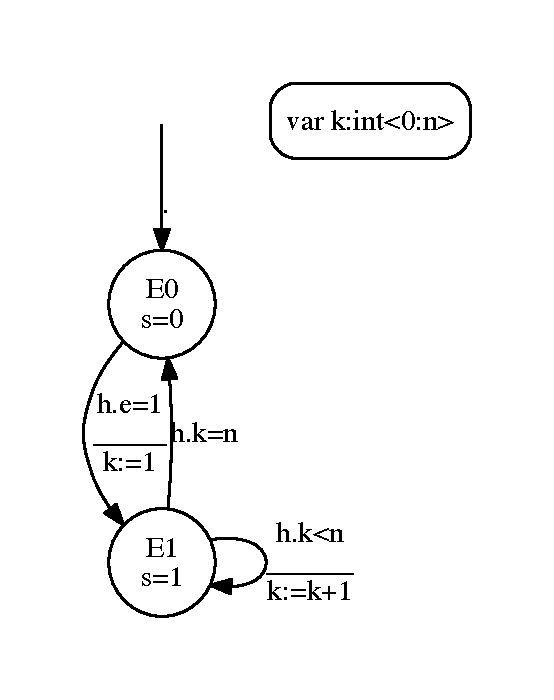
\includegraphics[height=9cm]{figs/gensig-model}
   \centering
  \caption{A graphical representation of FSM model defined in Listing~\ref{lst:rfsm-gensig}}
  \label{fig:rfsm-gensig-model}
\end{figure}

Note that, at this level, the value of the parameter \verb|n|, used in the type of the internal
variable \verb|k| (line~\ref{gensig-3}) and in the transition conditions (lines \ref{gensig-4} and
\ref{gensig-5}) is left unspecified, making the \verb|gensig| model a \emph{generic} one.

\medskip The second part of the program (lines \ref{gensig-2a}--\ref{gensig-2b}) lists \textbf{global inputs and
  outputs}.
% \footnote{In case of multi-FSM programs, this part will also contains the declaration of
%   \emph{shared} events and variables. See Sec.~\ref{sec:globals}.}.
For global outputs the
declaration simply gives a name and a type.  For global inputs, the declaration also specifies the
\textbf{stimuli} which are attached to the corresponding input for simulating the system. The
program of Listing~\ref{lst:rfsm-gensig} uses two kinds of stimuli\footnote{See
  Sec.~\ref{sec:inputs-outputs} for a complete description of stimuli.}. The stimuli attached to input
\verb|H| are declared as \emph{periodic}, with a period of 10 time units, a start time of 0 and a
end time of 80. This means than an event will be produced on this input at time 0, 10, 20, 30, 40,
50, 60, 70 and 80. The stimuli attached to input \verb|E| say that this input will respectively take
value 0, 1 and 0 at time 0, 25 and 35 (thus producing a ``pulse'' of duration 10 time units starting
at time 25).

\medskip
The third and last part of the program (line~\ref{gensig-6}) consists in building the global model of the system by
\emph{instanciating} the FSM model(s).
Instanciating a model creates a ``copy'' of this model for which
\begin{itemize}
\item the generic parameters (\verb|n| here) are now bound to actual values (3 here),
\item the inputs and outputs are connected to the global inputs or outputs. 
\end{itemize}

\medskip
A graphical representation of the system described in Listing~\ref{lst:rfsm-gensig} is given in
Fig.~\ref{fig:rfsm-gensig-top}\footnote{Again, this representation was actually automatically generated from the
program in Listing~\ref{lst:rfsm-gensig}, as explained in Chap.~\ref{cha:rfsmc}.}. 

\begin{figure}[!h]
   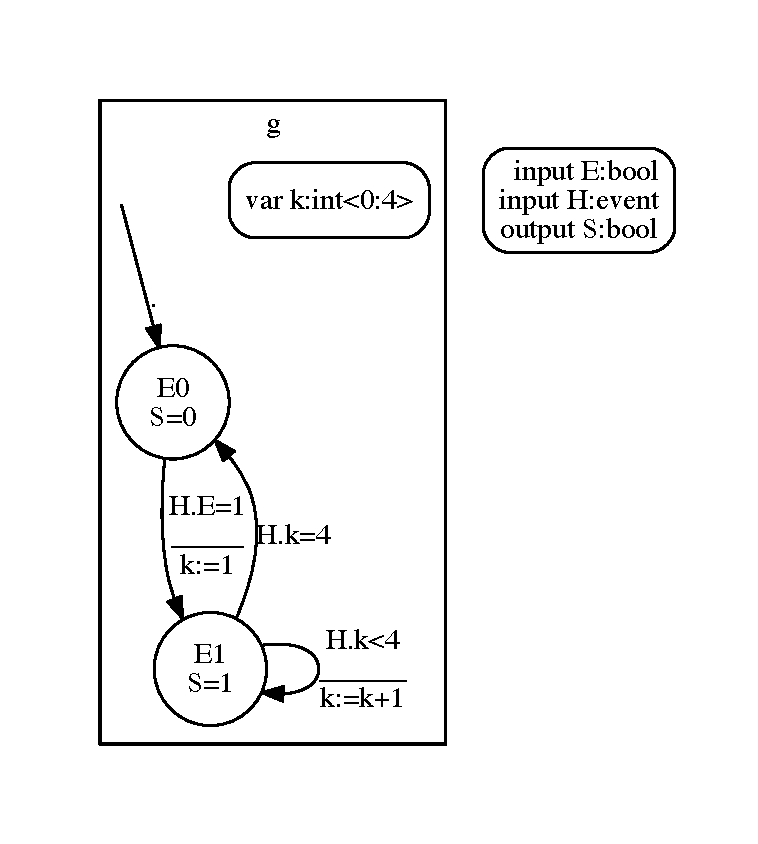
\includegraphics[height=7cm]{figs/gensig-top}
   \centering
  \caption{A graphical representation of system described in Listing~\ref{lst:rfsm-gensig}}
  \label{fig:rfsm-gensig-top}
\end{figure}

\section*{Simulating}
\label{sec:simulating-1}

Simulating the program means computing the reaction of the system to the input stimuli. Simulation
can be performed by the RFSM command-line compiler as described in chapter~\ref{cha:rfsmc}.
It produces a set of
\emph{traces} in VCD (Value Change Dump) format which can visualized using \emph{waveform viewers}
such as \texttt{gtkwave}. Some simulation results for the program in Listing~\ref{lst:rfsm-gensig}
are showed in Fig.~\ref{fig:rfsm-gensig-chrono}.

\begin{figure}[!h]
   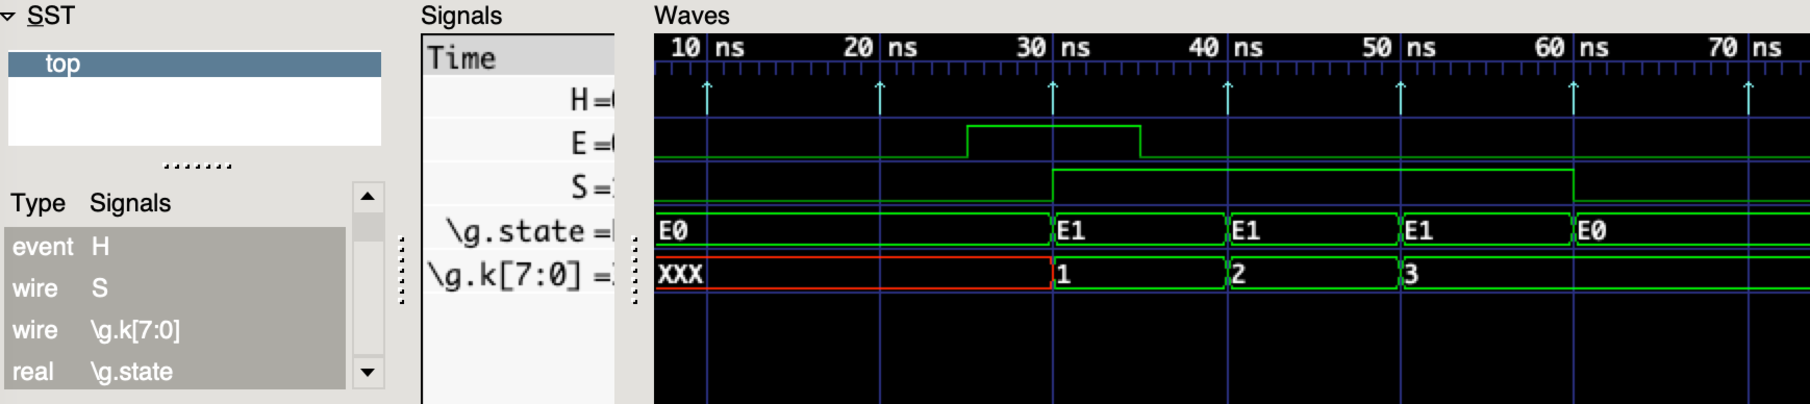
\includegraphics[width=\textwidth]{figs/gensig-chrono}
   \centering
  \caption{Simulation results for the program in Listing~\ref{lst:rfsm-gensig}, viewed using
    \texttt{gtkwave}}
  \label{fig:rfsm-gensig-chrono}
\end{figure}

\section*{Code generation}
\label{sec:code-generation-1}

RFSM can also generate code implementing the described systems simulation and/or
integration to existing applications.

\medskip
Currently, three backends are provided :
\begin{itemize}
\item a backend generating a C-based implementation of each FSM instance,
\item a backend generating a \emph{testbench} implementation in SystemC (FSM instances + stimuli
  generators),
\item a backend generating a \emph{testbench} implementation in VHDL (FSM instances + stimuli
  generators).
\end{itemize}

\medskip
The target language for the C backend is a C-like language augmented with
\begin{itemize}
\item a \verb|task| keyword for naming generated behaviors,
\item \verb|in|, \verb|out| and \verb|inout| keywords for identifying inputs and outputs,
\item a builtin \verb|event| type,
\item primitives for handling events : \verb|wait_ev()|, \verb|wait_evs()| and
  \verb|notify_ev()|. 
\end{itemize}
The idea is that the generated code can be turned into an application for a multi-tasking operating
system by providing actual implementations of the corresponding constructs and primitives.

\medskip
For the SystemC and VHDL backends, the generated code can actually be compiled and executed for
simulation purpose and. The FSM implementations generated by the VHDL backend can also be
synthetized to be implemented on hardware using hardware-specific tools\footnote{We use the
  \textsc{quartus} toolchain from Intel/Altera.}. 

\medskip
Appendices C1, C2 and C3 respectively give the C and SystemC code generated from the example in
Listing~\ref{lst:rfsm-gensig}. 

\section*{Variant formulation}
\label{sec:variant-formulation}

In the automata described in Fig.~\ref{fig:rfsm-gensig-model} and Listing~\ref{lst:rfsm-gensig}, the
value of the \texttt{s} output is specified by indicating how it changes when transitions are taken
(including its initialisation). This is typical of a so-called \emph{Mealy}-style description.  In
some cases, it is possible -- and maybe simpler -- to indicate which value this output takes for
each state. A equivalent description of that given
in Listing~\ref{lst:rfsm-gensig} is obtained, for example, by specifying that \texttt{s} is 0
whenever the FSM is in state \texttt{E0} and 1 whenever it is in state \texttt{E1}.
This style of description, often called
\emph{Moore}-style, is illustrated in Fig.~\ref{fig:rfsm-gensig-moore}. The value of the \texttt{s}
output is here attached to states using the \texttt{where} clause in the declarations of states.

\begin{figure}[htbp]
  \centering
  \begin{tabular}[c]{cc}
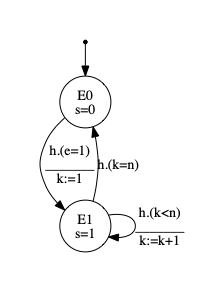
\includegraphics[width=0.4\textwidth]{figs/gensig-model-moore} &
\begin{minipage}[b]{0.6\textwidth}
\begin{lstlisting}[language=Rfsm]
fsm model gensig <n: int> (
  in h: event,
  in e: bool,
  out s: bool)
{
  states: E0 where s=0, E1 where s=1;
  vars: k: int<1:n>;
  trans:
  | E0 -> E1 on h when e=1 with k:=1
  | E1 -> E1 on h when k<n with k:=k+1
  | E1 -> E0 on h when k=n
  itrans:
 | -> E0 with s:=0
}
\end{lstlisting}
\end{minipage}
  \end{tabular}
  \caption{A reformulation of the model given in Listing~\ref{lst:rfsm-gensig} and
    Fig.~\ref{fig:rfsm-gensig-model} using Moore-style}
  \label{fig:rfsm-gensig-moore}
\end{figure}

\medskip \textbf{Note}. The \texttt{rfsmc} compiler automatically transforms models using
Moore-style descriptions models using only Mealy-style ones.

% This option is
% automatically inserted when simulating a system\footnote{\emph{I.e.} simulation is always performed
%   on Mealy-style FSMs.}. 

\section*{Multi-FSM models}
\label{sec:multi-fsm-models}

It is of course possible to describe systems composed of several FSM instances.

\medskip
A first example is given in Listing~\ref{lst:rfsm-cntmod8} and Fig.~\ref{fig:rfsm-cntmod8}. The system is a simple modulo 8 counter, here
described as a combination of three event-synchronized modulo 2 counters\footnote{This program is
  provided in the distribution, under directory \texttt{examples/std/multi/ctrmod8}.}.

Here a single FSM model (\texttt{cntmod2}) is instanciated thrice, as \texttt{C0}, \texttt{C1} and
\texttt{C2}. These instances are synchronized using two \textbf{shared events}, \texttt{R0} and \texttt{R1}. 
Shared events perform \emph{instantaneous synchronisation}. When a FSM \emph{emits} such an event, all transitions
triggered by this event are taken, simultaneously with the emitting transition. In the system
described in Fig.~\ref{fig:rfsm-cntmod8}, for example, the transition of \texttt{C0}
(resp. \texttt{C1}) from \texttt{E1} to \texttt{E0} occurs triggers the simultaneous transition of
\texttt{C1} (resp. \texttt{C2) }from \texttt{E0} to \texttt{E1} and, latter of \texttt{C1}
(resp. \texttt{C2}) from \texttt{E1} to \texttt{E0}.

\begin{figure}
  \centering
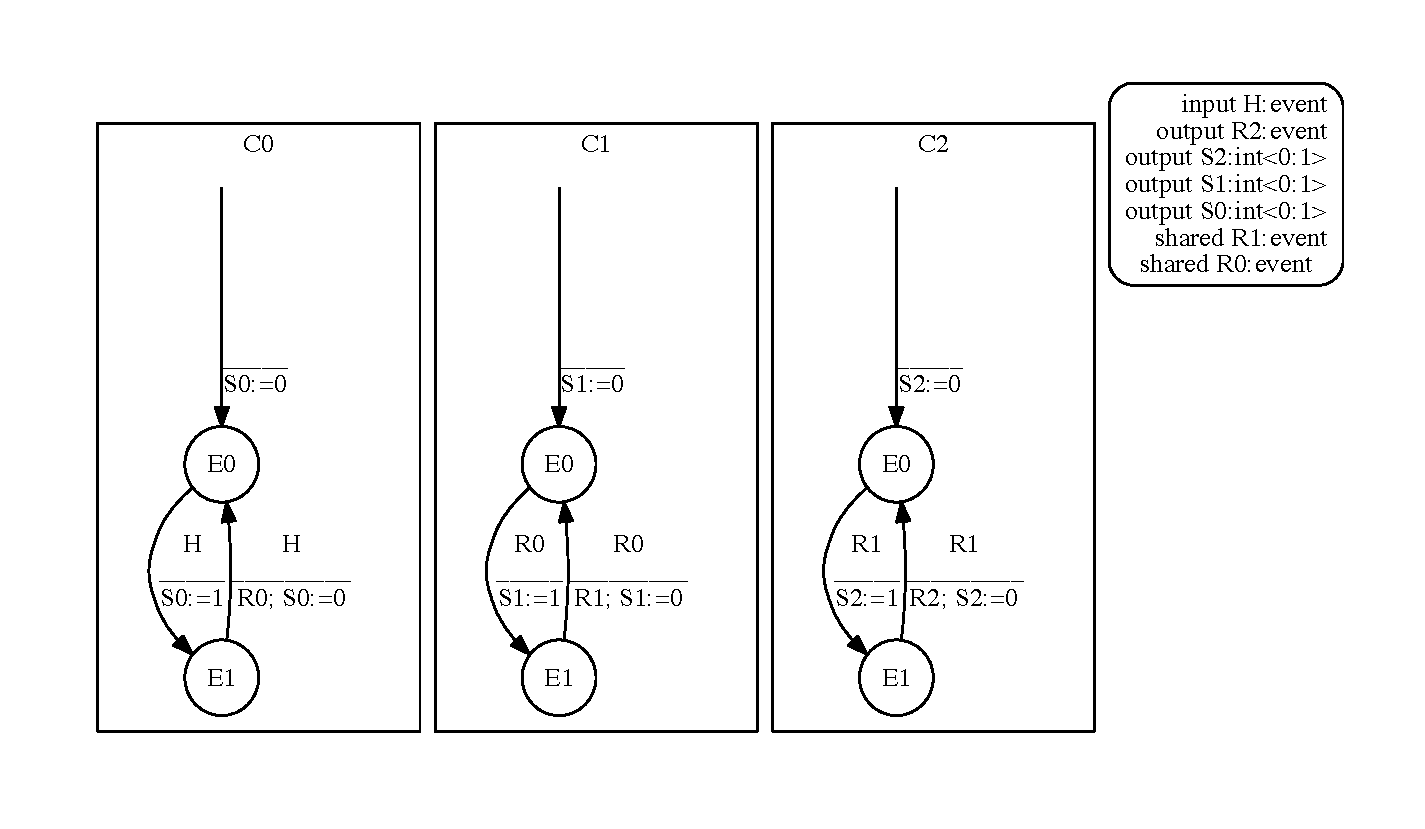
\includegraphics[width=\textwidth]{figs/ctrmod8-top}
  \caption{Graphical representation of the program of Listing~\ref{lst:rfsm-cntmod8}}
  \label{fig:rfsm-cntmod8}
\end{figure}

\begin{minipage}[c]{0.95\textwidth}
\begin{lstlisting}[frame=single,language=Rfsm,
  caption={A program involving three FSM instances synchronized by a shared event},
  label={lst:rfsm-cntmod8}]
fsm model cntmod2(
  in h: event,
  out s: bool,
  out r: event)
{
  states: E0 where s=0, E1 where s=1;
  trans:
  | E0 -> E1 on h
  | E1 -> E0 on h with r;
  itrans:
  | -> E0;
}

input H: event = periodic(10,10,100)
output S0, S1, S2: bool
output R2: event
shared R0, R1: event

fsm C0 = cntmod2(H,S0,R0) 
fsm C1 = cntmod2(R0,S1,R1) 
fsm C2 = cntmod2(R1,S2,R2) 
\end{lstlisting}
\end{minipage}

\pagebreak
Simulation results for this program are given in Fig.~\ref{fig:rfsm-cntmod8-vcd}.

\begin{figure}
   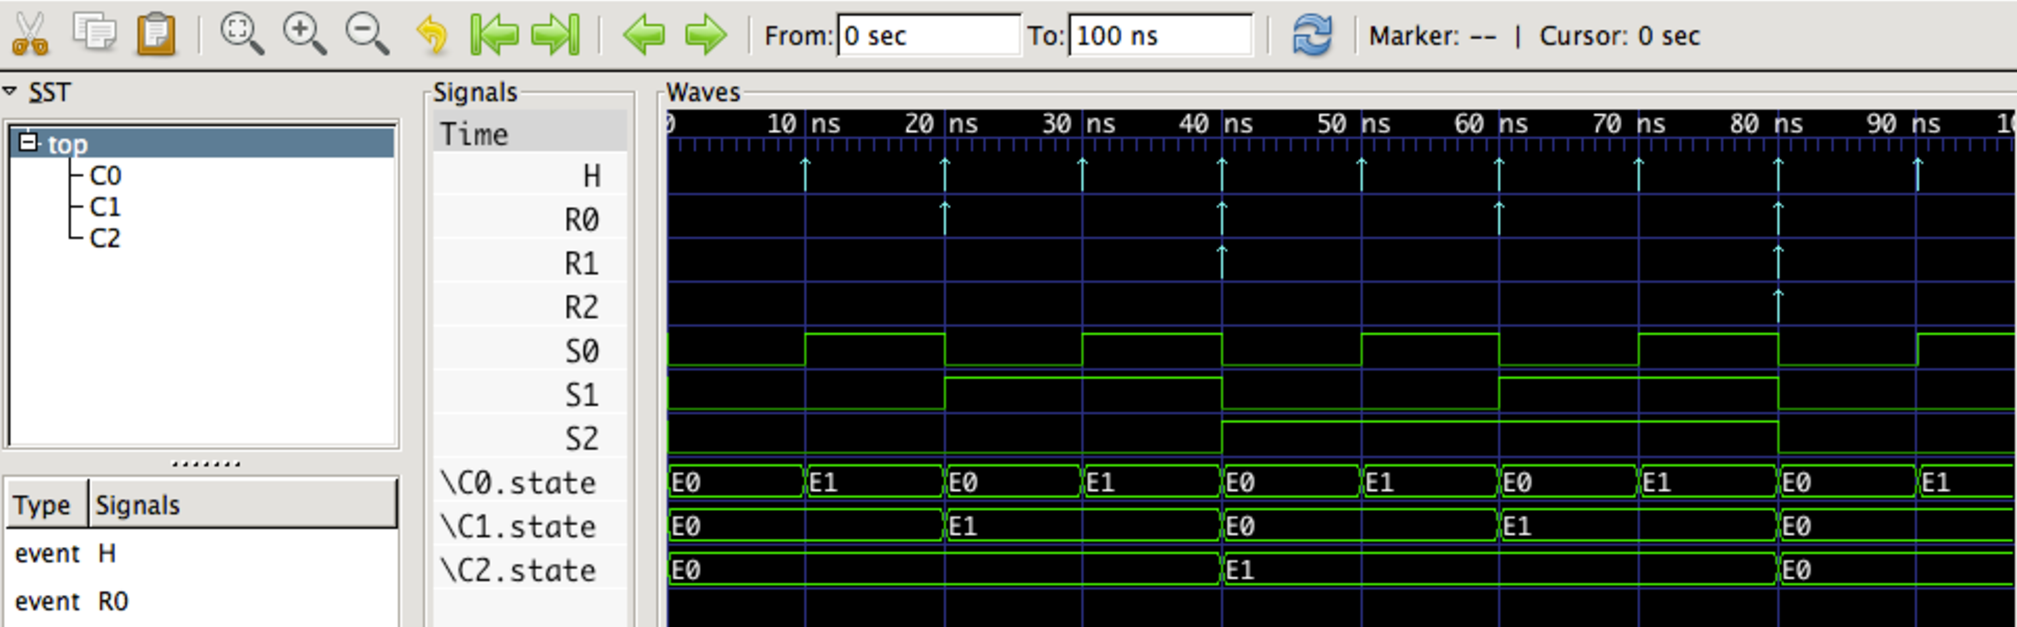
\includegraphics[width=0.9\textwidth]{figs/ctrmod8-chrono}
   \centering
  \caption{Simulation results for the program in Listing~\ref{fig:rfsm-cntmod8}}
  \label{fig:rfsm-cntmod8-vcd}
\end{figure}

\bigskip FSM instances can also interact by means of \textbf{shared variables}. This is illustrated
in Listing~\ref{lst:rfsm-shvar} and Fig.~\ref{fig:rfsm-shvar}\footnote{This program is provided in
  the distribution, under directory \texttt{examples/multi/synv_vp/ex5}.}. FSM \texttt{a1}
repeatedly writes the shared variable \texttt{c} at each event \texttt{h} so that it takes values 1,
2, 3, 4, 1, 2, \emph{etc}. FSM \texttt{a2} observes this variable also at each event \texttt{h} and
simply goes from state \texttt{S1} to state \texttt{S2} (resp. \texttt{S2} to \texttt{S1}) when the
observed value is 4 (resp. 1).

\begin{lstlisting}[frame=single,language=Rfsm,caption={A program involving two FSM instances and a
    shared variable},label={lst:rfsm-shvar}]
fsm model A1( in h: event, inout v: int)
{
  states: S1, S2;
  trans:
  | S1 -> S2 on h with v:=1
  | S2 -> S2 on h when v<4 with v:=v+1
  | S2 -> S1 on h when v=4;
  itrans:
  | -> S1 with v:=0;
}

fsm model A2( in h: event, in v: int)
{
  states: S1, S2;
  trans:
  | S1 -> S2 on h when v=4
  | S2 -> S1 on h when v=1;
  itrans:
  | -> S1 ;
}

input h : event = periodic(10,10,100)
shared c : int
fsm a1 = A1(h,c)
fsm a2 = A2(h,c)
\end{lstlisting}

\begin{figure}
  \centering
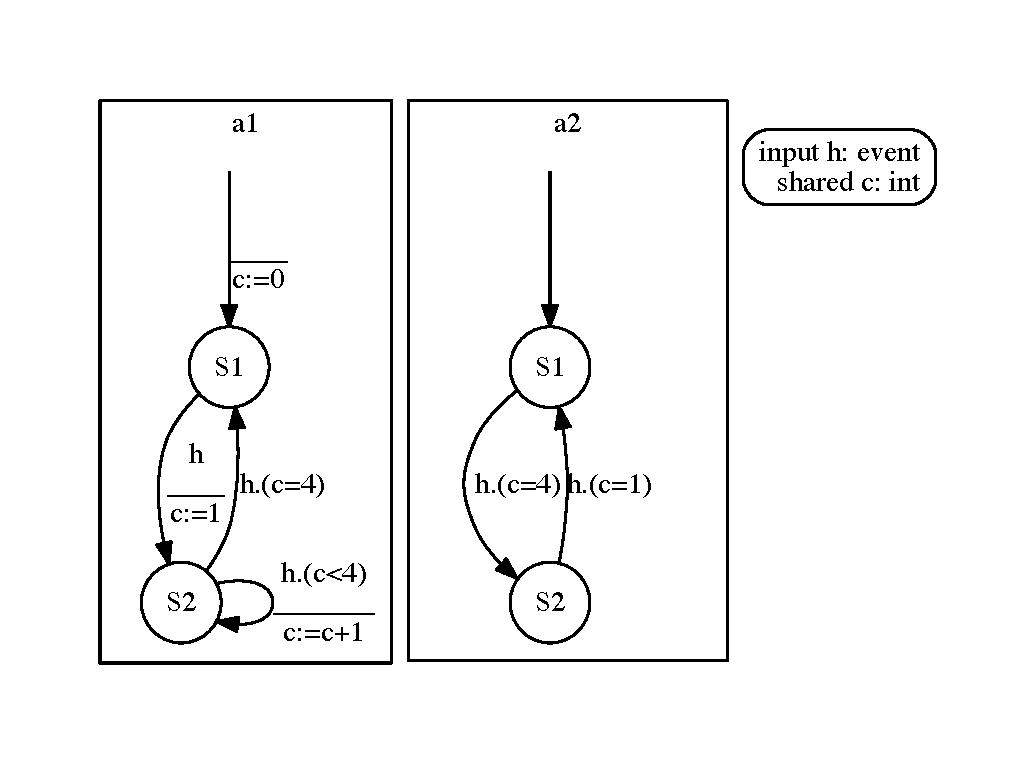
\includegraphics[width=0.8\textwidth]{figs/shvar-top} 
  \caption{Graphical representation of the program of Listing~\ref{lst:rfsm-shvar}}
  \label{fig:rfsm-shvar}
\end{figure}

Simulation results for this program are given in Fig.~\ref{fig:rfsm-shvar-vcd}.

\begin{figure}
   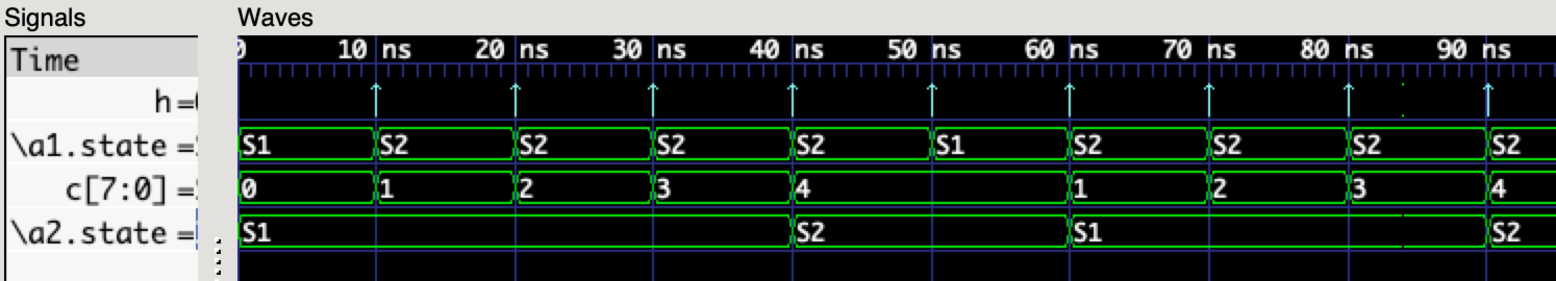
\includegraphics[width=0.95\textwidth]{figs/shvar-chrono}
   \centering
  \caption{Simulation results for the program in Listing~\ref{fig:rfsm-shvar}}
  \label{fig:rfsm-shvar-vcd}
\end{figure}


%%% Local Variables: 
%%% mode: latex
%%% TeX-master: "rfsm_um"
%%% End: 
   
\chapter{Using the RFSM compiler}
\label{cha:rfsmc}

The RFSM compiler can be used to
\begin{itemize}
\item produce graphical representations of FSM models and programs (using the \verb|.dot| format),
\item simulate programs, generating execution traces (\verb|.vcd| format),
\item generate C, SystemC or VHDL code from FSM models and programs.
\end{itemize}

This chapter describes how to invoke compiler on the command-line. On Unix systems, this is
done from a terminal running a shell interpreter. On Windows, from an MSYS or Cygwin
terminal.

\medskip
The compiler is invoked with a command like :

%rfsmc [options] file\textsubscript{1} ... file\textsubscript{n}
\begin{FVerbatim}[commandchars=\\\{\}]
rfsmc [options] \emph{source_files}
\end{FVerbatim}

\medskip
There must be at least one source file. If several are given, all happens as if a single one,
obtained by concatening all of them, in the given order, was used. 

\medskip
The complete set of options is described in App.~\ref{cha:compiler-options}.

\medskip
The set of generated files depends on the selected target. The output file \texttt{rfsm.output}
contains the list of the generated file.

\section{Generating graphical representations}
\label{sec:gener-graph-repr}

%rfsmc -dot f\textsubscript{1}.fsm ... f\textsubscript{n}.fsm
\begin{FVerbatim}[commandchars=\\\{\}]
rfsmc [-options] -dot \emph{source_files}
\end{FVerbatim}

The previous command generates a graphical representation of each FSM model 
contained in the given source file(s). If the source file(s) contain(s) FSM instances, involving global IOs
and shared objects, it also generates a graphical representation of the the corresponding system. 

The graphical representations use the \verb|.dot| format and can be viewed
with the \texttt{Graphviz} suite of tools\footnote{Available freely from
  \texttt{http://www.graphviz.org}.}.

The representation for the FSM model \verb|m| is generated in file \verb|m.dot|. When generated, the representation
for the system is written in file \verb|main.dot| by default. The name of this file can be changed
with the \verb|-main| option.

By default, the generated \verb|.dot| files are written in the current directory. This can be changed with the
\verb|-target_dir| option.

\section{Running the simulator}
\label{sec:running-simulator}

\begin{FVerbatim}[commandchars=\\\{\}]
rfsmc [-options] -sim \emph{source_files}
\end{FVerbatim}

The previous command runs simulator on the program described in the given source files, writing
an execution trace in VCD (Value Change Dump) format.

The generated \verb|.vcd| file can be viewed using a VCD visualizing application such as
\verb|gtkwave|\footnote{gtkwave.sourceforge.net}.

By default, the VCD file is named \verb|main.vcd|. This name can be changed using the \verb|-main| option.

By default, the VCD file is written in the current directory. This can be changed with the
\verb|-target_dir| option.

\section{Generating C code}
\label{sec:gener-c-code}

\begin{FVerbatim}[commandchars=\\\{\}]
rfsmc [-options] -ctask \emph{source_files}
\end{FVerbatim}

For each FSM model \verb|m| contained in the listed source file(s), the previous command generates a file
\verb|m.c| containing a C-based implementation of the corresponding behavior.

By default, the generated code is written in the current directory. This can be changed with the
\verb|-target_dir| option.

\section{Generating SystemC code}
\label{sec:gener-syst-code}

\begin{FVerbatim}[commandchars=\\\{\}]
rfsmc [-options] -systemc \emph{source_files}
\end{FVerbatim}

If the source file(s) only contain(s) FSM \emph{models}, then, for each listed FSM model \texttt{m}, 
the previous command generates a pair of files \verb|m.h| and \verb|m.cpp| containing the
  interface and implementation of the SystemC module implementing this model.

\medskip
If the source file(s) contain(s) FSM \emph{instances}, involving global IOs
and shared objects, it generates
\begin{itemize}
\item for each FSM instance \verb|m|, a pair of files \verb|m.h| and \verb|m.cpp| containing the
  interface and implementation of the SystemC module implementing this instance,
\item for each global input \verb|i|, a pair of files \verb|inp_i.h|
  and \verb|inp_i.cpp| containing the interface and implementation of the SystemC module describing
  this input (generating the associated stimuli, in particular),
\item a file \verb|main.cpp| containing the description of the \emph{testbench} for simulating the
  program.
\end{itemize}

The name of the file containing the \emph{testbench} can be changed with the \verb|main| option.

\medskip
By default, the generated code is written in the current directory. This can be changed with the
\verb|-target_dir| option.

\medskip
Simulation itself is performed by compiling the generated code and running the executable,
using the standard SystemC toolchain.
In order to simplify this, the RFSM compiler also generates a list of \emph{Makefile} targets to be
appended to a predefined \emph{Makefile} so that compiling and running the code generated by the
SystemC backend can be performed by simply invoking \verb|make| on this \emph{Makefile}. For this,
the RFSM compiler simply needs to know where this predefined \emph{Makefile} has been
installed. This is achieved by using the \verb|-lib| option when invoking the compiler. For example,
provided that RFSM has been installed in directory \verb|/usr/local/rfsm|, the following command

\begin{FVerbatim}[commandchars=\\\{\}]
rsfmc -systemc -lib /usr/local/rfsm/lib -target_dir ./systemc \emph{source_file(s)}
\end{FVerbatim}

will write in directory \verb|./systemc| the generated source files and the corresponding
\verb|Makefile|. Compiling these files and running the resulting application is then simply achieved
by typing

\begin{verbatim}
cd ./systemc
make 
\end{verbatim}

\medskip
\textbf{Note}. Of course, you may have to adjust some definitions in the file
\verb|.../lib/etc/Makefile.systemc| to reflect the specificities of your local SystemC installation. 

\section{Generating VHDL code}
\label{sec:generating-vhdl-code}

\begin{FVerbatim}[commandchars=\\\{\}]
rfsmc [-options] -vhdl \emph{source_files}
\end{FVerbatim}

If the source file(s) only contain(s) FSM \emph{models}, then, for each listed FSM model \texttt{m}, 
the previous command generates file \verb|m.vhd| containing the entity and architecture describing
this model.

\medskip
If the source file(s) contain(s) FSM \emph{instances}, involving global IOs
and shared objects, it generates
\begin{itemize}
\item for each FSM instance \verb|m|, a file \verb|m.vhd| containing an entity and architecture
  description for this instance,
\item a file \verb|main_top.vhd| containing the description of the \emph{top level} model of the
  system,
\item a file \verb|main_tb.vhd|containing the description of the \emph{testbench} for
  simulating the system.
\end{itemize}

\medskip The name of the files containing the \emph{top level} description \emph{testbench} can be
changed with the \verb|main| option.

\medskip
By default, the generated code is written in the current directory. This can be changed with the
\verb|-target_dir| option.

\medskip
The produced files can then compiled, simulated and synthetized using a standard VHDL
toolchain\footnote{We use GHDL for simulation and Altera/Quartus for synthesis.}.

Concerning simulation, and as for the SystemC backend, the process can be grealy simplified by using
a pair of \emph{Makefile}s, one predefined and the other generated by the compiler.  For example,
and, again, provided that RFSM has been installed in directory \verb|/usr/local/rfsm|, the following
command

\begin{FVerbatim}[commandchars=\\\{\}]
rsfmc -vhdl -lib /usr/local/rfsm/lib -target_dir ./vhdl \emph{source_file(s)}
\end{FVerbatim}

will write in directory \verb|./vhdl| the generated source files and the corresponding
\verb|Makefile|. Compiling these files and running the resulting application is then simply achieved
by typing

\begin{verbatim}
cd ./vhdl
make 
\end{verbatim}

\medskip
\textbf{Note}. As for the SystemC backend, for this to work, you may have to adjust some definitions in the file

\section{Using \texttt{make}}
\label{sec:makefile}

The current distribution provides, in \verb|.../lib/etc| directory, a file \verb|Makefile.app|
aiming at easing the invokation of the RFSM compiler and the exploitation of the generated
products.

Suppose, for instance, that RFSM has been installed in \verb|/usr/local/rfsm| and the application is
to be compiled is made of two source files, \verb|foo.fsm|, containing the FSM model(s), and
\verb|main.fsm|, containing the global declarations and FSM instanciations (the so-called
\emph{testbench}). The only thing to do is create the following Makefile in the working directory
(that containing the RFSM source file)

\begin{lstlisting}[language=make,frame=single]
TB=main
SRCS=foo.fsm main.fsm
DOT_OPTS= ...
SIM_OPTS= ...
SYSTEMC_OPTS= ...
VHDL_OPTS= ...
include /usr/local/rfsm/lib/etc/Makefile.app
\end{lstlisting}

Then, simply typing\footnote{Please refer to the file \texttt{Makefile.app} itself for
  a complete list of targets.}
  \begin{itemize}
  \item \verb|make dot| will generate the \verb|.dot| and lauch the corresponding viewer,
  \item \verb|make sim.run| to run the simulation using the interpreter (\verb|make sim.show| to display results),
  \item \verb|make ctask.code| will invoke the C backend C and generate the corresponding code,
  \item \verb|make systemc.code| will invoke the SystemC backend  and generate the corresponding code,
  \item \verb|make systemc.run| will invoke the SystemC backend, generate the corresponding
    code, compile it and run the corresponding simulation,
  \item \verb|make vhdl.code| will invoke the VHDL backend  and generate the corresponding code,
  \item \verb|make vhdl.run| will invoke the VHDL backend, generate the corresponding
    code, compile it and run the corresponding simulation,
  \item \verb|make sim.show| (resp \verb|make systemc.show| and \verb|make vhdl.show|) will display
    the simulation traces generated by the interpreter (resp. SystemC and VHDL simulation).
  \end{itemize}


%%% Local Variables: 
%%% mode: latex
%%% TeX-master: "rfsm"
%%% End: 

\chapter{ Formal syntax of RFSM programs}
\label{cha:bnf}

This appendix gives a BNF definition of the concrete syntax RFSM programs.
As stated in the introduction, this syntax is that of the so-called \emph{standard} RFSM language.
Variant languages will essentially differ in the definition of the
$\rfsmtypedecl*{}$,
$\rfsmtypeexpr*{}$,
$\rfsmexpr*{}$,
$\rfsmconstant*{}$,
and $\rfsmconst*{}$
syntactical categories.

\medskip
The meta-syntax is conventional. Keywords are written in \textbf{boldface}.  Non-terminals are
enclosed in angle brackets ({\tt <} \ldots {\tt >}).  Vertical bars ({\tt |}) indicate
alternatives.  Constructs enclosed in non-bold brackets ({\tt [} \ldots {\tt ]}) are optional.
The notation $E^*$ (resp $E^+$) means zero (resp one) or more repetitions of $E$, separated by spaces.
The notation $E^*_x$ (resp $E^+_x$) means zero (resp one) or more repetitions of $E$, separated by
symbol $x$. Terminals \verb|lid| and \verb|uid| respectively designate identifiers
starting with a lowercase and uppercase letter. 

\begin{rfsmgrammar}
\rfsmgramfunc{\rfsmprogram{}}& \rfsmgramdef & \rfsmgramstar{\rfsmtypedecl*{}} \\ & &
                                              \rfsmgramstar{\rfsmcstdecl*{}} \\ & &
                                              \rfsmgramstar{\rfsmfndecl*{}} \\ & &
                                              \rfsmgramstar{\rfsmfsmmodel*{}} \\ & &
                                              \rfsmgramstar{\rfsmfsmmodel*{}} \\ & &
                                              \rfsmgramstar{\rfsmglobal*{}} \\ & &
                                              \rfsmgramstar{\rfsmfsminst*{}}
                                              \rfsmEOF*{}
  \\& & \\

\rfsmgramfunc{\rfsmtypedecl{}}& \rfsmgramdef & \rfsmTYPE*{} \rfsmLID*{}
                                               \rfsmEQUAL*{} \rfsmtypeexpr*{}\\
  & \rfsmgrambar &\rfsmTYPE*{} \rfsmLID*{} \rfsmEQUAL*{} \rfsmENUM*{}
                  \rfsmbraced{\rfsmgramseplist{\rfsmCOMMA*{}}{\rfsmUID*{}}}\\
  & \rfsmgrambar &\rfsmTYPE*{} \rfsmLID*{} \rfsmEQUAL*{} \rfsmRECORD*{}
                  \rfsmLBRACE*{}
                  \rfsmgramsepnelist{\rfsmCOMMA*{}}{\rfsmrecordfield*{}}
                  \rfsmRBRACE*{}
  \\& & \\

\rfsmgramfunc{\rfsmrecordfield{}}& \rfsmgramdef & \rfsmLID*{} \rfsmCOLON*{}
                                                  \rfsmtypeexpr*{}
  \\& & \\

\rfsmgramfunc{\rfsmcstdecl{}}& \rfsmgramdef & \rfsmCONSTANT*{} \rfsmLID*{}
                                              \rfsmCOLON*{} \rfsmtypeexpr*{}
                                              \rfsmEQUAL*{} \rfsmconst*{}
  \\& & \\

\rfsmgramfunc{\rfsmfndecl{}}& \rfsmgramdef & \rfsmFUNCTION*{} \rfsmLID*{}
                                             \rfsmLPAREN*{}
                                             \rfsmgramseplist{\rfsmCOMMA*{}}{\rfsmfarg*{}}
                                             \rfsmRPAREN*{} \rfsmCOLON*{}
                                             \rfsmtypeexpr*{} \rfsmLBRACE*{}
                                             \rfsmRETURN*{} \rfsmexpr*{}
                                             \rfsmRBRACE*{}
  \\& & \\

\rfsmgramfunc{\rfsmfarg{}}& \rfsmgramdef & \rfsmLID*{} \rfsmCOLON*{}
                                           \rfsmtypeexpr*{}
  \\& & \\

\rfsmgramfunc{\rfsmfsmmodel{}}& \rfsmgramdef & \rfsmFSM*{} \rfsmMODEL*{}
                                               \rfsmid*{}
                                               \rfsmgramopt{\rfsmparams*{}}
                                               \rfsmLPAREN*{}
                                               \rfsmgramseplist{\rfsmCOMMA*{}}{\rfsmio*{}}
                                               \rfsmRPAREN*{} \rfsmLBRACE*{} \\ & &
                                               \rfsmSTATES*{} \rfsmCOLON*{}
                                               \rfsmgramseplist{\rfsmCOMMA*{}}{\rfsmstate*{}}
                                               \rfsmSEMICOLON*{} \\ & &
                                               \rfsmgramopt{\rfsmvars*{}} \\ & &
                                               \rfsmTRANS*{} \rfsmCOLON*{}
                                               \rfsmgramseplist{\rfsmCOMMA*{}}{\rfsmtransition*{}}
                                               \rfsmSEMICOLON*{} \\ & &
                                               \rfsmITRANS*{} \rfsmCOLON*{}
                                               \rfsmitransition*{}
                                               \rfsmSEMICOLON*{} \\ & &
                                               \rfsmRBRACE*{}
  \\& & \\

  \rfsmgramfunc{\rfsmstate{}}& \rfsmgramdef & \rfsmUID*{}
                                              \rfsmgramopt{\rfsmWHERE \rfsmgramsepnelist{\rfsmAND{}}{\rfsmoutpval*{}}}

  \\& & \\
\rfsmgramfunc{\rfsmoutpval{}}& \rfsmgramdef & \rfsmLID*{} \rfsmEQUAL*{} \rfsmscalarconst*{}


  \\& & \\

\rfsmgramfunc{\rfsmparams{}}& \rfsmgramdef & \rfsmLT*{}
                                             \rfsmgramseplist{\rfsmCOMMA*{}}{\rfsmparam*{}}
                                             \rfsmGT*{}
  \\& & \\

\rfsmgramfunc{\rfsmparam{}}& \rfsmgramdef & \rfsmLID*{} \rfsmCOLON*{}
                                            \rfsmtypeexpr*{}
  \\& & \\

\rfsmgramfunc{\rfsmio{}}& \rfsmgramdef & \rfsmIN*{} \rfsmiodesc*{}\\
  & \rfsmgrambar &\rfsmOUT*{} \rfsmiodesc*{}\\
  & \rfsmgrambar &\rfsmINOUT*{} \rfsmiodesc*{}
  \\& & \\

\rfsmgramfunc{\rfsmiodesc{}}& \rfsmgramdef & \rfsmLID*{} \rfsmCOLON*{}
                                             \rfsmtypeexpr*{}
  \\& & \\

\rfsmgramfunc{\rfsmvars{}}& \rfsmgramdef & \rfsmVARS*{} \rfsmCOLON*{}
                                           \rfsmgramseplist{\rfsmCOMMA*{}}{\rfsmvar*{}}
                                           \rfsmSEMICOLON*{}
  \\& & \\

\rfsmgramfunc{\rfsmvar{}}& \rfsmgramdef & \rfsmgramsepnelist{\rfsmCOMMA*{}}{\rfsmLID*{}}
                                          \rfsmCOLON*{} \rfsmtypeexpr*{}
  \\& & \\

\rfsmgramfunc{\rfsmtransition{}}& \rfsmgramdef & \rfsmrulepfx*{}
                                                 \rfsmUID*{}
                                                 \rfsmARROW*{}
                                                 \rfsmUID*{}
                                                 \rfsmcondition*{}
                                                 \rfsmgramopt{\rfsmactions*{}}
  \\& & \\

  \rfsmgramfunc{\rfsmrulepfx{}}& \rfsmgramdef & \rfsmBAR*{} \rfsmgrambar \rfsmEMARK*{}

  \\& & \\

\rfsmgramfunc{\rfsmcondition{}}& \rfsmgramdef & \rfsmON*{} \rfsmLID*{} \rfsmgramopt{\rfsmguards*{}} \\

  \\& & \\

\rfsmgramfunc{\rfsmguards{}}& \rfsmgramdef & \rfsmWHEN*{} \rfsmgramsepnelist{\rfsmDOT*{}}{\rfsmexpr*{}}

  \\& & \\

\rfsmgramfunc{\rfsmactions{}}& \rfsmgramdef & \rfsmWITH*{} \rfsmgramsepnelist{\rfsmSEMICOLON*{}}{\rfsmaction*{}}
  \\& & \\

\rfsmgramfunc{\rfsmaction{}}& \rfsmgramdef & \rfsmLID*{}\\
  & \rfsmgrambar &\rfsmlhs*{} \rfsmCOLEQ*{} \rfsmexpr*{}
  \\& & \\

\rfsmgramfunc{\rfsmlhs{}}& \rfsmgramdef & \rfsmLID*{}\\
  & \rfsmgrambar &\rfsmLID*{} \rfsmLBRACKET*{} \rfsmexpr*{} \rfsmRBRACKET*{}\\
  & \rfsmgrambar &\rfsmLID*{} \rfsmLBRACKET*{} \rfsmexpr*{} \rfsmCOLON*{}
                  \rfsmexpr*{} \rfsmRBRACKET*{}\\
  & \rfsmgrambar &\rfsmLID*{} \rfsmDOT*{} \rfsmLID*{}
  \\& & \\

  \rfsmgramfunc{\rfsmitransition{}}& \rfsmgramdef & \rfsmBAR*{} \rfsmARROW*{} \rfsmUID*{} \rfsmgramopt{\rfsmactions*{}}
                                                  
  \\& & \\

\rfsmgramfunc{\rfsmglobal{}}& \rfsmgramdef & \rfsmINPUT*{} \rfsmid*{}
                                             \rfsmCOLON*{} \rfsmtypeexpr*{}
                                             \rfsmEQUAL*{} \rfsmstimuli*{}\\
  & \rfsmgrambar &\rfsmOUTPUT*{}
                  \rfsmgramsepnelist{\rfsmCOMMA*{}}{\rfsmid*{}} \rfsmCOLON*{}
                  \rfsmtypeexpr*{}\\
  & \rfsmgrambar &\rfsmSHARED*{}
                  \rfsmgramsepnelist{\rfsmCOMMA*{}}{\rfsmid*{}} \rfsmCOLON*{}
                  \rfsmtypeexpr*{}
  \\& & \\

\rfsmgramfunc{\rfsmstimuli{}}& \rfsmgramdef & \rfsmPERIODIC*{} \rfsmLPAREN*{}
                                              \rfsmINT*{} \rfsmCOMMA*{}
                                              \rfsmINT*{} \rfsmCOMMA*{}
                                              \rfsmINT*{} \rfsmRPAREN*{}\\
  & \rfsmgrambar &\rfsmSPORADIC*{}
                  \rfsmparen{\rfsmgramseplist{\rfsmCOMMA*{}}{\rfsmINT*{}}}\\
  & \rfsmgrambar &\rfsmVALUECHANGES*{}
                  \rfsmparen{\rfsmgramseplist{\rfsmCOMMA*{}}{\rfsmvaluechange*{}}}
  \\& & \\

\rfsmgramfunc{\rfsmvaluechange{}}& \rfsmgramdef & \rfsmINT*{} \rfsmCOLON*{}
                                                  \rfsmstimconst*{}
  \\& & \\

\rfsmgramfunc{\rfsmfsminst{}}& \rfsmgramdef & \rfsmFSM*{} \rfsmid*{}
                                              \rfsmEQUAL*{} \rfsmid*{}
                                              \rfsmgramopt{\rfsmLT*{}
                                              \rfsmgramsepnelist{\rfsmCOMMA*{}}{\rfsmparamvalue*{}}
                                              \rfsmGT*{}}
                                              \rfsmparen{\rfsmgramseplist{\rfsmCOMMA*{}}{\rfsmid*{}}}
  \\& & \\

\rfsmgramfunc{\rfsmparamvalue{}}& \rfsmgramdef & \rfsmscalarconst*{}\\
  & \rfsmgrambar &\rfsmLID*{}

  \\& & \\

\rfsmgramfunc{\rfsmtypeexpr{}}& \rfsmgramdef & \rfsmTYEVENT*{}\\
  & \rfsmgrambar &\rfsmTYINT*{} \rfsmintannot*{}\\
  & \rfsmgrambar &\rfsmTYFLOAT*{}\\
  & \rfsmgrambar &\rfsmTYCHAR*{}\\
  & \rfsmgrambar &\rfsmTYBOOL*{}\\
  & \rfsmgrambar &\rfsmLID*{}\\
  & \rfsmgrambar &\rfsmtypeexpr*{} \rfsmTYARRAY*{} \rfsmLBRACKET*{}
                  \rfsmarraysize*{} \rfsmRBRACKET*{}
  \\& & \\

\rfsmgramfunc{\rfsmintannot{}}& \rfsmgramdef & \rfsmgrameps \\
  & \rfsmgrambar &\rfsmLT*{} \rfsmtypesize*{} \rfsmGT*{}\\
  & \rfsmgrambar &\rfsmLT*{} \rfsmtypesize*{} \rfsmCOLON*{}
                  \rfsmtypesize*{} \rfsmGT*{}
  \\& & \\

\rfsmgramfunc{\rfsmarraysize{}}& \rfsmgramdef & \rfsmtypesize*{}
  \\& & \\

\rfsmgramfunc{\rfsmtypesize{}}& \rfsmgramdef & \rfsmINT*{}\\
  & \rfsmgrambar &\rfsmLID*{}\\

  \\& & \\

\rfsmgramfunc{\rfsmexpr{}}& \rfsmgramdef & \rfsmsimpleexpr*{}\\
  & \rfsmgrambar &\rfsmexpr*{} \rfsmPLUS*{} \rfsmexpr*{}\\
  & \rfsmgrambar &\rfsmexpr*{} \rfsmMINUS*{} \rfsmexpr*{}\\
  & \rfsmgrambar &\rfsmexpr*{} \rfsmTIMES*{} \rfsmexpr*{}\\
  & \rfsmgrambar &\rfsmexpr*{} \rfsmDIV*{} \rfsmexpr*{}\\
  & \rfsmgrambar &\rfsmexpr*{} \rfsmMOD*{} \rfsmexpr*{}\\
  & \rfsmgrambar &\rfsmexpr*{} \rfsmEQUAL*{} \rfsmexpr*{}\\
  & \rfsmgrambar &\rfsmexpr*{} \rfsmNOTEQUAL*{} \rfsmexpr*{}\\
  & \rfsmgrambar &\rfsmexpr*{} \rfsmGT*{} \rfsmexpr*{}\\
  & \rfsmgrambar &\rfsmexpr*{} \rfsmLT*{} \rfsmexpr*{}\\
  & \rfsmgrambar &\rfsmexpr*{} \rfsmGTE*{} \rfsmexpr*{}\\
  & \rfsmgrambar &\rfsmexpr*{} \rfsmLTE*{} \rfsmexpr*{}\\
  & \rfsmgrambar &\rfsmexpr*{} \rfsmLAND*{} \rfsmexpr*{}\\
  & \rfsmgrambar &\rfsmexpr*{} \rfsmLOR*{} \rfsmexpr*{}\\
  & \rfsmgrambar &\rfsmexpr*{} \rfsmLXOR*{} \rfsmexpr*{}\\
  & \rfsmgrambar &\rfsmexpr*{} \rfsmSHR*{} \rfsmexpr*{}\\
  & \rfsmgrambar &\rfsmexpr*{} \rfsmSHL*{} \rfsmexpr*{}\\
  & \rfsmgrambar &\rfsmexpr*{} \rfsmFPLUS*{} \rfsmexpr*{}\\
  & \rfsmgrambar &\rfsmexpr*{} \rfsmFMINUS*{} \rfsmexpr*{}\\
  & \rfsmgrambar &\rfsmexpr*{} \rfsmFTIMES*{} \rfsmexpr*{}\\
  & \rfsmgrambar &\rfsmexpr*{} \rfsmFDIV*{} \rfsmexpr*{}\\
  & \rfsmgrambar &\rfsmsubtractive*{} \rfsmexpr*{}\\
  & \rfsmgrambar &\rfsmLID*{} \rfsmLBRACKET*{} \rfsmexpr*{} \rfsmRBRACKET*{}\\
  & \rfsmgrambar &\rfsmLID*{} \rfsmLBRACKET*{} \rfsmexpr*{} \rfsmCOLON*{}
                  \rfsmexpr*{} \rfsmRBRACKET*{}\\
  & \rfsmgrambar &\rfsmLID*{} \rfsmLPAREN*{}
                  \rfsmgramseplist{\rfsmCOMMA*{}}{\rfsmexpr*{}}
                  \rfsmRPAREN*{}\\
  & \rfsmgrambar &\rfsmLID*{} \rfsmDOT*{} \rfsmLID*{}\\
  & \rfsmgrambar &\rfsmexpr*{} \rfsmQMARK*{} \rfsmexpr*{} \rfsmCOLON*{}
                  \rfsmexpr*{}\\
  & \rfsmgrambar &\rfsmexpr*{} \rfsmCOLONCOLON*{} \rfsmtypeexpr*{}
  \\& & \\

\rfsmgramfunc{\rfsmsimpleexpr{}}& \rfsmgramdef & \rfsmLID*{}\\
  & \rfsmgrambar &\rfsmUID*{}\\
  & \rfsmgrambar &\rfsmscalarconst*{}\\
  & \rfsmgrambar &\rfsmLPAREN*{} \rfsmexpr*{} \rfsmRPAREN*{}
  \\& & \\

\rfsmgramfunc{\rfsmsubtractive{}}& \rfsmgramdef & \rfsmMINUS*{}\\
  & \rfsmgrambar &\rfsmFMINUS*{}
  \\& & \\

\rfsmgramfunc{\rfsmscalarconst{}}& \rfsmgramdef & \rfsmINT*{}\\
  & \rfsmgrambar &\rfsmBOOL*{}\\
  & \rfsmgrambar &\rfsmFLOAT*{}\\
  & \rfsmgrambar &\rfsmCHAR*{}
  \\& & \\

\rfsmgramfunc{\rfsmconst{}}& \rfsmgramdef & \rfsmscalarconst*{}\\
  & \rfsmgrambar &\rfsmarrayconst*{}\\
  \\& & \\

\rfsmgramfunc{\rfsmarrayconst{}}& \rfsmgramdef & \rfsmLBRACKET*{}
                                                 \rfsmgramsepnelist{\rfsmCOMMA*{}}{\rfsmconst*{}}
                                                 \rfsmRBRACKET*{}
  \\& & \\

\rfsmgramfunc{\rfsmstimconst{}}& \rfsmgramdef & \rfsmscalarconst*{}\\
  & \rfsmgrambar &\rfsmscalarconst*{} \rfsmCOLONCOLON*{} \rfsmtypeexpr*{}\\
  & \rfsmgrambar & \rfsmUID*{}\\
  & \rfsmgrambar & \rfsmrecordconst*{}\
  \\& & \\

\rfsmgramfunc{\rfsmrecordconst{}}& \rfsmgramdef & \rfsmLBRACE*{}
                                                  \rfsmgramsepnelist{\rfsmCOMMA*{}}{\rfsmrecordfieldconst*{}}
                                                  \rfsmRBRACE*{}
  \\& & \\

\rfsmgramfunc{\rfsmrecordfieldconst{}}& \rfsmgramdef & \rfsmLID*{}
                                                       \rfsmEQUAL*{}
                                                       \rfsmstimconst*{}
  \\& & \\

\rfsmgramfunc{\rfsmid{}}& \rfsmgramdef & \rfsmLID*{}\\
  & \rfsmgrambar &\rfsmUID*{}
  \\& & \\

\end{rfsmgrammar}

%%% Local Variables: 
%%% mode: latex
%%% TeX-master: "rfsm_rm"
%%% End: 


%%% Local Variables:
%%% mode: latex
%%% TeX-master: "rfsm"
%%% End:

\chapter*{Appendix B - Compiler options}
\label{cha:compiler-options}

Compiler usage : \verb|rfsmc [options...] files|

\medskip
\begin{tabular}[c]{ll}
-lib & set location of the support library (default: /usr/local/rfsm/lib)\\
-dump\_model & dump model in text format to stdout\\
-target\_dir & set target directory (default: .)\\
-dot & generate top-level .dot representation(s)\\
-sim & run simulation (generating .vcd file)\\
-ctask & generate CTask code\\
-systemc & generate SystemC code\\
-vhdl & generate VHDL code\\
-version & print version of the compiler and quit\\
-dot\_no\_captions & Remove captions in .dot representation(s)\\
-dot\_fsm\_insts & generate .dot representation of all FSM instances\\
-dot\_fsm\_models & generate .dot representation of all FSM models\\
-dot\_actions\_nl & write actions with with a separating newline\\
-trace & set trace level for simulation (default: 0)\\
-vcd & set name of .vcd output file when running simulation (default: run.vcd)\\
-synchronous\_actions & interpret actions synchronously\\
-sc\_time\_unit & set time unit for the SystemC test-bench (default: SC\_NS)\\
-sc\_trace & set trace mode for SystemC backend (default: false)\\
-stop\_time & set stop time for the SystemC and VHDL test-bench (default: 100)\\
-sc\_double\_float & implement float type as C++ double instead of float (default: false)\\
-vhdl\_trace & set trace mode for VHDL backend (default: false)\\
-vhdl\_time\_unit & set time unit for the VHDL test-bench\\
-vhdl\_ev\_duration & set duration of event signals (default: 1 ns)\\
-vhdl\_rst\_duration & set duration of reset signals (default: 1 ns)\\
-vhdl\_numeric\_std & translate integers as numeric\_std [un]signed (default: false)\\
-vhdl\_bool\_as\_bool & translate all booleans as boolean (default: false)\\

\end{tabular}

\normalsize

%%% Local Variables: 
%%% mode: latex
%%% TeX-master: "rfsm"
%%% End: 

\chapter*{Appendix C1 - Example of generated C code}  
\label{cha:ex1-c}

This is the code generated from program given in Listing~\ref{lst:rfsm-gensig} 

\begin{lstlisting}[language=ctask,frame=single,numbers=none,basicstyle=\small]
task g(
  in event h;
  in int e;
 out int s;
  )
{
  int k;
  enum {E0,E1} state = E0;
  s=0;
  while ( 1 ) {
    switch ( state ) {
    case E1:
      wait_ev(h);
      if ( k<4 ) {
        k=k+1;
        }
      else if ( k==4 ) {
        s=0;
        state = E0;
        }
      break;
    case E0:
      wait_ev(h);
      if ( e==1 ) {
        k=1;
        s=1;
        state = E1;
        }
      break;
    }
  }
};
\end{lstlisting}
%%% Local Variables: 
%%% mode: latex
%%% TeX-master: "rfsm"
%%% End: 

\chapter*{Appendix C1 - Example of generated SystemC code}  
\label{cha:ex1-systemc}

This is the code generated from program given in Listing~\ref{lst:rfsm-example} 

\begin{lstlisting}[language=systemc,frame=single,numbers=none,basicstyle=\small,caption=File c1.h]
#include "systemc.h"

SC_MODULE(C1)
{
  // Types
  typedef enum { Idle, Wait } t_state;
  // IOs
  sc_in<bool> Top;
  sc_in<bool> Clic;
  sc_out<bool> SimpleClic;
  sc_out<bool> DoubleClic;
  sc_out<int> st;
  // Constants
  static const int D = 5;
  // Local variables
  t_state state;
  int ctr;

  void react();

  SC_CTOR(C1) {
    SC_THREAD(react);
    }
};
\end{lstlisting}

\begin{lstlisting}[language=systemc,frame=single,numbers=none,basicstyle=\small,caption=File c1.cpp]
#include "c1.h"
#include "rfsm.h"

void C1::react()
{
  state = Idle;
  while ( 1 ) {
    st = state;
    switch ( state ) {
    case Wait:
      wait(Top.posedge_event() | Clic.posedge_event());
      if ( Top.read() ) {
        if ( ctr<4 ) {
          ctr=ctr+1;
          }
        else if ( ctr==4 ) {
          notify_ev(SimpleClic,"SimpleClic");
          state = Idle;
          }
        }
      else if ( Clic.read() ) {
        notify_ev(DoubleClic,"DoubleClic");
        state = Idle;
        }
      wait(SC_ZERO_TIME);
      break;
    case Idle:
      wait(Clic.posedge_event());
      ctr=0;
      state = Wait;
      wait(SC_ZERO_TIME);
      break;
    }
  }
};
\end{lstlisting}

\begin{lstlisting}[language=systemc,frame=single,numbers=none,basicstyle=\small,caption=File
  inp_Clic.h]
#include "systemc.h"

SC_MODULE(Inp_Clic)
{
  // Output
  sc_out<bool> Clic;

  void gen();

  SC_CTOR(Inp_Clic) {
    SC_THREAD(gen);
    }
};
\end{lstlisting}

\begin{lstlisting}[language=systemc,frame=single,numbers=none,basicstyle=\small,caption=File
  inp_Clic.cpp]
#include "inp_Clic.h"
#include "rfsm.h"

static int _dates[3] = { 25, 75, 95 };

void Inp_Clic::gen()
{
  int _i=0, _t=0;
  while ( _i < 3 ) {
    wait(_dates[_i]-_t, SC_NS);
    notify_ev(Clic,"Clic");
    _t = _dates[_i];
    _i++;
    }
};
\end{lstlisting}

\begin{lstlisting}[language=systemc,frame=single,numbers=none,basicstyle=\small,caption=File inp_Clk.h]
#include "systemc.h"

SC_MODULE(Inp_Clk)
{
  // Output
  sc_out<bool> Clk;

  void gen();

  SC_CTOR(Inp_Clk) {
    SC_THREAD(gen);
    }
};
\end{lstlisting}

\begin{lstlisting}[language=systemc,frame=single,numbers=none,basicstyle=\small,caption=File
  inp_Clk.cpp]
#include "inp_Clk.h"
#include "rfsm.h"

typedef struct { int period; int t1; int t2; } _periodic_t;

static _periodic_t _clk = { 10, 10, 120 };

void Inp_Clk::gen()
{
  int _t=0;
  wait(_clk.t1, SC_NS);
  notify_ev(Clk,"Clk");
  _t = _clk.t1;
  while ( _t <= _clk.t2 ) {
    wait(_clk.period, SC_NS);
    notify_ev(Clk,"Clk");
    _t += _clk.period;
    }
};
\end{lstlisting}

\begin{lstlisting}[language=systemc,frame=single,numbers=none,basicstyle=\small,caption=File tb.cpp]
#include "systemc.h"
#include "rfsm.h"
#include "inp_Clic.h"
#include "inp_Clk.h"
#include "c1.h"

int sc_main(int argc, char *argv[])
{
  sc_signal<bool> Clic;
  sc_signal<bool> Clk;
  sc_signal<bool> DClic;
  sc_signal<bool> SClic;
  sc_signal<int> c1_state;
  sc_trace_file *trace_file;
  trace_file = sc_create_vcd_trace_file ("tb");
  sc_trace(trace_file, Clic, "Clic");
  sc_trace(trace_file, Clk, "Clk");
  sc_trace(trace_file, DClic, "DClic");
  sc_trace(trace_file, SClic, "SClic");
  sc_trace(trace_file, c1_state, "c1_state");

  Inp_Clic Inp_Clic("Inp_Clic");
  Inp_Clic(Clic);
  Inp_Clk Inp_Clk("Inp_Clk");
  Inp_Clk(Clk);

  C1 c1("c1");
  c1(Clk,Clic,SClic,DClic,c1_state);

  sc_start(120, SC_NS);

  sc_close_vcd_trace_file (trace_file);

  return EXIT_SUCCESS;
}
\end{lstlisting}

%%% Local Variables: 
%%% mode: latex
%%% TeX-master: "rfsm"
%%% End: 

\chapter*{Appendix A3 - Example of generated VHDL code}  
\label{cha:ex1-vhdl}

This is the code generated from program given in Listing~\ref{lst:rfsm-gensig} by the VHDL backend.

\begin{lstlisting}[language=VHDL,frame=single,numbers=none,basicstyle=\small,caption=File g.vhd]
library ieee;
use ieee.std_logic_1164.all;
use work.rfsm.all;

entity G is
  port( H: in std_logic;
        E: in std_logic;
        S: out std_logic;
        rst: in std_logic
        );
end entity;

architecture RTL of G is
  type t_state is ( E0, E1 );
  signal state: t_state;
begin
  process(rst, H)
  variable k: integer;
  begin
    if ( rst='1' ) then
      state <= E0;
      S <= '0';
    elsif rising_edge(H) then 
      case state is
      when E0 =>
        if ( E = '1' ) then
          k := 1;
          S <= '1';
          state <= E1;
        end if;
      when E1 =>
        if ( k = 3 ) then
          S <= '0';
          state <= E0;
        elsif  ( k<3 ) then
          k := k+1;
        end if;
    end case;
    end if;
  end process;
end architecture;

\end{lstlisting}

\begin{lstlisting}[language=VHDL,frame=single,numbers=none,basicstyle=\small,caption=File main_top.vhd]
library ieee;
use ieee.std_logic_1164.all;	   

entity main_top is
  port(
        H: in std_logic;
        E: in std_logic;
        S: out std_logic;
        rst: in std_logic        );
end entity;

architecture struct of main_top is

component G 
  port(
        H: in std_logic;
        E: in std_logic;
        S: out std_logic;
        rst: in std_logic
        );
end component;


begin
  G0: G port map(H,E,S,rst);
end architecture;
\end{lstlisting}

\begin{lstlisting}[language=VHDL,frame=single,numbers=none,basicstyle=\small,caption=File main_tb.vhd]
library ieee;
use ieee.std_logic_1164.all;	   

use work.rfsm.all;
entity main_tb is
end entity;

architecture struct of main_tb is

component main_top is
  port(
        H: in std_logic;
        E: in std_logic;
        S: out std_logic;
        rst: in std_logic        );
end component;

signal H: std_logic;
signal E: std_logic;
signal S: std_logic;
signal rst: std_logic;

begin

  inp_H: process
    type t_periodic is record period: time; t1: time; t2: time; end record;
    constant periodic : t_periodic := ( 10 ns, 10 ns, 80 ns );
    variable t : time := 0 ns;
    begin
      H <= '0';
      wait for periodic.t1;
      t := t + periodic.t1;
      while ( t < periodic.t2 ) loop
        H <= '1';
        wait for periodic.period/2;
        H <= '0';
        wait for periodic.period/2;
        t := t + periodic.period;
      end loop;
      wait;
  end process;
  inp_E: process
    type t_vc is record date: time; val: std_logic; end record;
    type t_vcs is array ( 0 to 2 ) of t_vc;
    constant vcs : t_vcs := ( (0 ns,'0'), (25 ns,'1'), (35 ns,'0') );
    variable i : natural := 0;
    variable t : time := 0 ns;
    begin
      for i in 0 to 2 loop
        wait for vcs(i).date-t;
        E <= vcs(i).val;
        t := vcs(i).date;
      end loop;
      wait;
  end process;
  reset: process
  begin
    rst <= '1';
    wait for 1 ns;
    rst <= '0';
    wait for 100 ns;
    wait;
  end process;

  Top: main_top port map(H,E,S,rst);

end architecture;

\end{lstlisting}

%%% Local Variables: 
%%% mode: latex
%%% TeX-master: "rfsm_um"
%%% End: 


% \input{source}
% \input{biblio}

\bibliographystyle{plain}
\bibliography{rfsm}

\end{document}

%%% Local Variables:
%%% mode: latex
%%% TeX-master: t
%%% End:
